\documentclass[11pt]{article}
\usepackage[a4paper,margin=0.8in]{geometry}
\usepackage{amsmath,amssymb}
\usepackage{graphicx}
\usepackage[colorlinks=true,linkcolor=blue,citecolor=blue,urlcolor=blue]{hyperref}
\newcommand{\JJ}{\mathcal J}
\newcommand{\BB}{\mathcal B}

\title{Why BFKL comes with $\log\frac{\vee}{k^+}$ and JIMWLK with $\log\frac{\vee}{\Lambda}$}
\date{}

\begin{document}
\maketitle

\paragraph{Which logarithm goes with which evolution.}
The extra (unobserved or virtual) gluon that produces the leading logarithms has plus momentum $p^+$ in the window $\Lambda<p^+<\vee$. Here $\vee$ is the plus momentum of the valence charges $\rho$ of the projectile, and $\Lambda$ is the cutoff below which gluons are counted as part of the target. The measured gluon, with plus momentum $k^+$, splits this window into two parts,
\begin{equation}
\log\frac{\vee}{\Lambda}=\log\frac{\vee}{k^+}+\log\frac{k^+}{\Lambda}.
\end{equation}
A large logarithm arises only when $p^+$ is strongly ordered with respect to $k^+$, and the two orderings are physically different (Fig.~\ref{fig:rap}). Plus momentum is conserved at every splitting, so a gluon can only be emitted by a parent with larger $p^+$. Equivalently, in light-cone time the lifetime of a fluctuation, $x^+\sim 2p^+/p_\perp^2$, grows with $p^+$: harder gluons are formed earlier and softer ones later, closer to the target.
\begin{itemize}
\item $k^+\ll p^+<\vee$. The extra gluon is harder than the measured one.
\begin{itemize}
\item It is already part of the projectile wave function when the measured gluon is formed, and it can itself emit the measured gluon ($\rho\to p^+\to k^+$).
\item Together with the corresponding virtual terms this is the evolution of the projectile. For a dilute projectile it is linear: BFKL.
\item Its phase space is $\log\frac{\vee}{k^+}$.
\end{itemize}
\item $\Lambda<p^+\ll k^+$. The extra gluon is softer than the measured one.
\begin{itemize}
\item It is emitted by all harder charges, the valence charges and the measured gluon, just before the target. Its multiple scattering on the target is what the JIMWLK evolution of the target resums.
\item Its phase space is $\log\frac{k^+}{\Lambda}$.
\end{itemize}
\end{itemize}
The BFKL terms in which the measured gluon is emitted by the extra gluon (23 of the 35 terms of BFKL$\otimes$LO) exist only for $p^+>k^+$. In the explicit calculation they come from the upper limits $p^+\to\vee$ of the $p^+$ integrals and appear only with $\log\frac{\vee}{k^+}$. They cannot carry $\log\frac{\vee}{\Lambda}$: that would include the region $p^+<k^+$, where a gluon softer than the measured one would have to emit it.

The terms in which both gluons are emitted by the valence charges (the JIMWLK structure) have the $p^+$ integral of the extra gluon over the whole window. Summing all rows of the $O(g^4)$ cross section gives (checked term by term for a general adjoint Wilson line $U$)
\begin{equation}
\frac{d^3N}{d^3k}\bigg|_{\rm LL}=\log\frac{\vee}{\Lambda}\;\JJ+\log\frac{\vee}{k^+}\,\big(\BB-\JJ\big),\qquad \JJ={\rm JIMWLK}\otimes{\rm LO},\quad \BB={\rm BFKL}\otimes{\rm LO}.
\label{eq:rows}
\end{equation}
The coefficient of the full interval $\log\frac{\vee}{\Lambda}$ is the JIMWLK term alone, and BFKL appears only with $\log\frac{\vee}{k^+}$. The $-\JJ\log\frac{\vee}{k^+}$ removes the JIMWLK term from the region $p^+>k^+$, where the projectile evolution (BFKL) takes over. Eq.~\eqref{eq:rows} is the same as
\begin{equation}
\frac{d^3N}{d^3k}\bigg|_{\rm LL}=\log\frac{k^+}{\Lambda}\;\JJ+\log\frac{\vee}{k^+}\;\BB,
\label{eq:fact}
\end{equation}
which is the standard rapidity factorization of single inclusive production: the projectile is evolved from $\vee$ down to $k^+$, the target from $\Lambda$ up to $k^+$~\cite{KT,BKNW,KL,KLW}.

Each extra gluon has one value of $p^+$, so the interval $\log\frac{\vee}{\Lambda}$ is shared between the two evolutions, not given to both. Writing $\log\frac{\vee}{\Lambda}(\JJ+\BB)$ would count the region $p^+>k^+$ twice. At mid rapidity, $k^+=\sqrt{\vee\Lambda}$, each evolution gets half of the window:
\begin{equation}
\frac{d^3N}{d^3k}\bigg|_{\rm LL}=\frac12\log\frac{\vee}{\Lambda}\,\big(\JJ+\BB\big)+\log\frac{k^+}{\sqrt{\vee\Lambda}}\,\big(\JJ-\BB\big).
\end{equation}
The last term is the distance in rapidity from the centre of the window. It vanishes at mid rapidity and does not grow with $\log\frac{\vee}{\Lambda}$.

\begin{figure}[h]
\centering
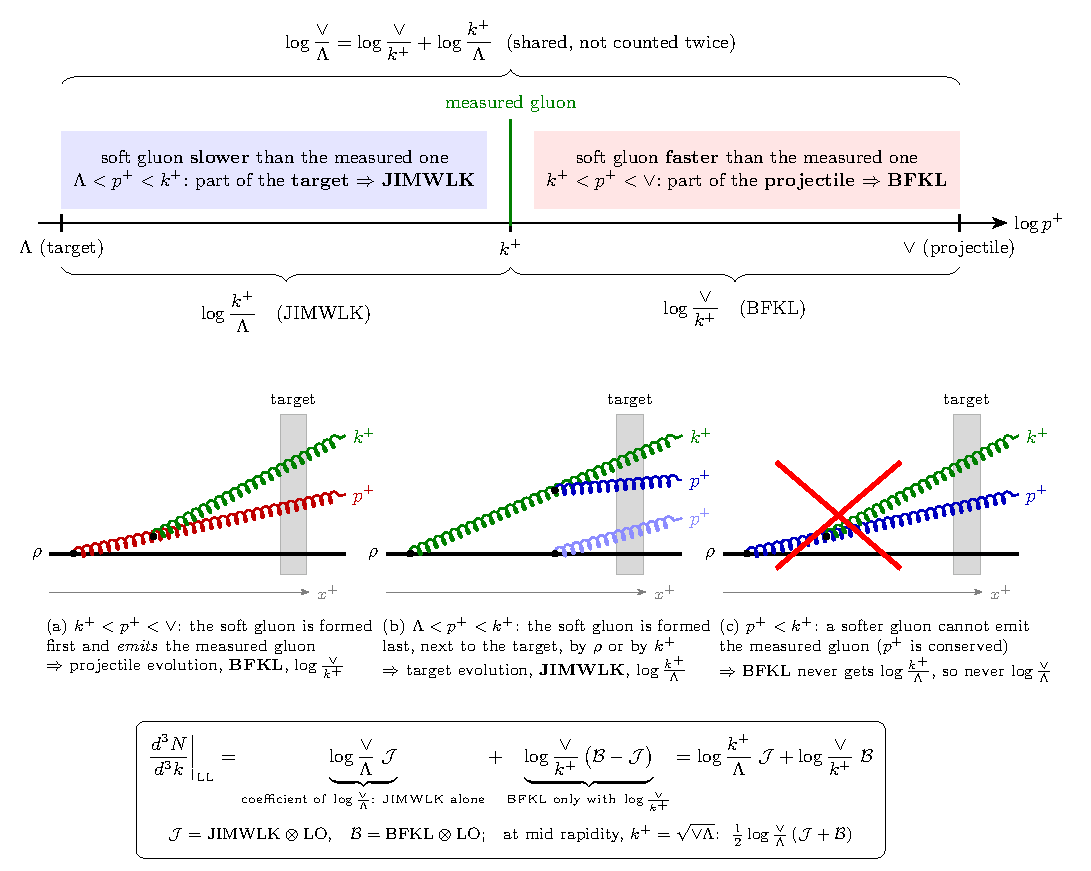
\includegraphics[width=\textwidth]{Rapidity_figure.pdf}
\caption{Top: the soft window $\Lambda<p^+<\vee$ is split by the measured gluon $k^+$. Gluons harder than $k^+$ belong to the projectile (BFKL, $\log\frac{\vee}{k^+}$), softer ones to the target (JIMWLK, $\log\frac{k^+}{\Lambda}$). Bottom: (a) the BFKL cascade $\rho\to p^+\to k^+$ needs $p^+>k^+$; (b) a softer gluon is emitted by $\rho$ or by the measured gluon, next to the target, and is part of the target evolution; (c) the measured gluon cannot be emitted by a softer gluon. Horizontal axis of the diagrams: light-cone time $x^+$; the grey band is the target.}
\label{fig:rap}
\end{figure}

\begin{thebibliography}{9}
\bibitem{KT} Yu.~V. Kovchegov and K.~Tuchin, ``Inclusive gluon production in DIS at high parton density,'' Phys.\ Rev.\ D \textbf{65}, 074026 (2002), \href{https://arxiv.org/abs/hep-ph/0111362}{hep-ph/0111362}.
\bibitem{BKNW} R.~Baier, A.~Kovner, M.~Nardi and U.~A. Wiedemann, ``Particle correlations in saturated QCD matter,'' Phys.\ Rev.\ D \textbf{72}, 094013 (2005), \href{https://arxiv.org/abs/hep-ph/0506126}{hep-ph/0506126}.
\bibitem{KL} A.~Kovner and M.~Lublinsky, ``One gluon, two gluon: multigluon production via high energy evolution,'' JHEP \textbf{11}, 083 (2006), \href{https://arxiv.org/abs/hep-ph/0609227}{hep-ph/0609227}.
\bibitem{KLW} A.~Kovner, M.~Lublinsky and H.~Weigert, ``Treading on the cut: semi inclusive observables at high energy,'' Phys.\ Rev.\ D \textbf{74}, 114023 (2006), \href{https://arxiv.org/abs/hep-ph/0608258}{hep-ph/0608258}.
\end{thebibliography}
\end{document}
